\documentclass{standalone}
\usepackage{tikz}
\usepackage{pgfplots}

\begin{document}
\def\gaussianTwoD#1#2#3{
  \pgfmathdeclarefunction{#1}{2}{
    \pgfmathparse{exp( -((##1 - #2)^2 + (##2-#3)^2 ))}
  }
}

\def\gaussianOneD#1#2{
  \pgfmathdeclarefunction{#1}{1}{\pgfmathparse{2.71^(-((##1 - #2)^2))}}
}
\gaussianOneD{mygaussian}{0}
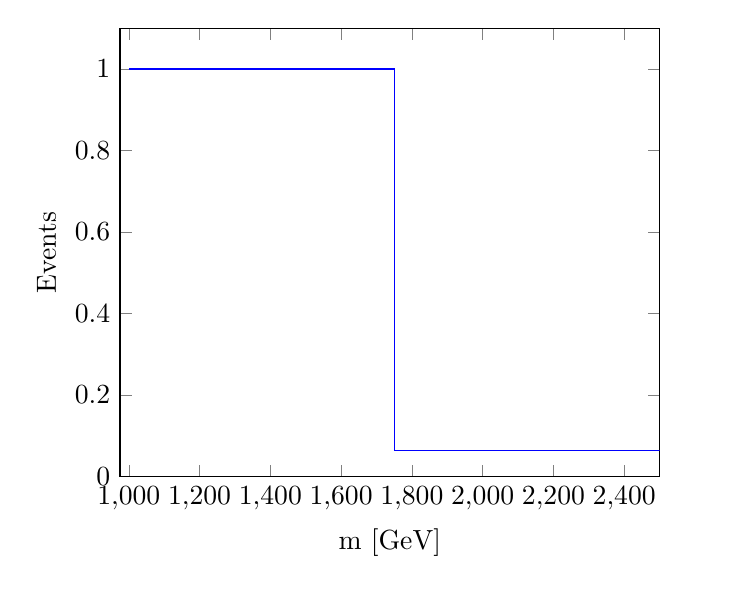
\begin{tikzpicture}
  \begin{axis}[
    ymin=0, ymax=1.1,
    xmin=975, xmax=2500,
    xlabel={m [GeV]},
    ylabel={Events},
    nodes near coords={\node (plot-\coordindex) at (axis cs:
\pgfkeysvalueof{/data point/x}, \pgfkeysvalueof{/data point/y}) {};}
    ]
    \addplot+[blue, const plot mark mid, domain=1000:2500, samples=2, mark=none] plot  {40^(-(x-1000)/2000)};
  \end{axis}

\end{tikzpicture}

\end{document}
